\documentclass[12pt,letterpaper]{article}
\usepackage{fullpage}
\usepackage[top=2cm, bottom=4.5cm, left=2.5cm, right=2.5cm]{geometry}
\usepackage{amsmath,amsthm,amsfonts,amssymb,amscd}
\usepackage{dsfont}
\usepackage{lastpage}
\usepackage{enumerate}
\usepackage{fancyhdr}
\usepackage{mathrsfs}
\usepackage{xcolor}
\usepackage{graphicx}
\usepackage{listings}
\usepackage[hyphens,spaces,obeyspaces]{url}
\usepackage{hyperref}
\usepackage{float}
\usepackage[export]{adjustbox}
\restylefloat{table}





\pagestyle{myheadings}
\markright{\hspace{17cm}}
\title{Optimized Conversion of Categorical and Numerical Features in Machine Learning Models}
\author{Tom Butler, Emily Liang, Wren Paris-Moe, Andrea Stine}

\theoremstyle{plain}
\newtheorem{theorem}{Theorem}[section]
\newtheorem{corollary}[theorem]{Corollary}
\newtheorem{lemma}[theorem]{Lemma}
\newtheorem{conjecture}[theorem]{Conjecture}
\newtheorem{example}[theorem]{Example}
\theoremstyle{definition}
\newtheorem{definition}[theorem]{Definition}


\begin{document}


\maketitle


\begin{abstract}
While some data have an explicit, numerical form, many other data, such as gender or nationality, do not typically use numbers and are referred to as categorical data. Thus, machine learning algorithms need a way of representing categorical information numerically in order to be able to analyze them. Our project specifically focuses on optimizing the conversion of categorical features to a numerical form in order to maximize the effectiveness of various machine learning models. Of the methods we used, we found that Wide \& Deep is the most effective model for datasets that contain high-cardinality features, as opposed to learned embedding and one-hot encoding. 
\end{abstract}


\section{Introduction}
\hspace{\parindent}Data come in a variety of types, though generally a piece of data falls into one of two types: numerical data and categorical data. These can be further broken down into ordinal and nominal data types for categorical features, and interval and ratio data types for numerical data \cite{datatypes}. 

Numerical data have precise numerical values with the connotation that numbers provide. Income, for example, is numerical data; it is sensible to talk about adding, subtracting from, multiplying, or dividing one's income, and for any two levels of income, we can always compare if one individual's income is higher than another individual's income \cite{numdata}.

Ordinal data, by contrast, have an order, but are not subject to mathematical operations. Often a survey will ask a subject to rate something from a set of options: ``Strongly disagree, disagree, neutral, agree, strongly agree," for example. The results provided by the subject are a case of ordinal data---able to be put in an order, but unable to be added to or subtracted from \cite{categdata}.

Lastly, nominal data have no order and also are not subject to mathematical operations. Gender, for example, is not ordered and is not subject to mathematical operations \cite{categdata}.

A machine learning algorithm has no issue interpreting numerical or ordinal data, since both are typically and most naturally represented with numbers. By contrast, a machine learning algorithm does not typically have a method of processing categorical data unless the categorical data have been provided numerical representations.

The simplest method of numerically representing categorical data is known as an ordinal representation: For a given feature, each option within the feature is assigned a whole number value. As an example, gender can be assigned with $\text{male} = 0$, $\text{female} = 1$, $\text{nonbinary} = 2$, $\text{unspecified} = 3$, or any other permutation of numbers with a particular option for gender \cite{ordinal}. 

One alternative to ordinal encoding of categorical features is one-hot encoding. For a categorical feature, one-hot encoding involves creating unit vectors for each option within the categorical feature, where the dimensionality of the vector equals the number of possibilities for the categorical feature. Thus, a possible one-hot encoding for gender, as above, could be $\text{male} = (1, 0, 0, 0)$, $\text{female} = (0, 1, 0, 0)$, $\text{nonbinary} = (0, 0, 1, 0)$, $\text{unspecified} = (0, 0, 0, 1)$. Each value that gender can take is given its own column in the vector, thus preventing the algorithm from weighting one over another \cite{gender}. 

Now, let's consider a scenario where your model internally calculates averages and your values for gender are ordinally encoded as $\text{male}=1$, $\text{female}=2$, $\text{nonbinary}=3$, $\text{unspecified}=4$. Thus, your model presupposes that $\text{male}>\text{female}>\text{nonbinary}>\text{unspecified}$. If it were to automatically calculate averages, you might encounter a problem where it averages $\text{male + nonbinary}=1+3=4$ to find that the average is $2$, which is also the encoded value for female. This would most likely lead to poor performance in outcome predictions and lead to unexpected predictions \cite{gender}. By providing each option with a unit vector, one-hot encoding resolves the issue of ordinal encoding. However, one-hot encoding can be slow if the categorical feature has a high cardinality. Further, in certain disciplines, such as natural language processing, it may be helpful for options within a categorical feature to have a connection to one another \cite{naturallang}. 

One example of when one-hot encoding is useful is with zip codes. Although zip codes are comprised of a numerical representation, they are simply a representation of a certain area \cite{zipcode}. Thus, when we encode our features, we encode them as categorical features rather than as numerical ones. Using one-hot encoding in this case will ensure that the algorithm does not weight one location over the others due to its numerical representation \cite{onehotencode}. However, because there are nearly 42,000 zipcodes in the U.S., this would create a vector of dimensionality $42,000 \times 1$, one-hot encoding is not very efficient because of the high cardinality of the features \cite{zipcodestat}. 

\subsection{The Problem}

\hspace{\parindent}Our primary problem that we were given was to find the best way to encode categorical data for machine learning algorithms. We were presented with six different datasets, and given different goals to accomplish for each. For example, the objective for the ``Adult" dataset was to predict which individuals made above \$50,000 a year. However, all the datasets consisted partially or entirely of categorical features, which we had to encode as numerical values before we were able to input them into any machine learning model. We explore the benefits and detriments of one-hot encoding, typical categorical encoders, learned embedding, as well as the Wide \& Deep model in categorical feature conversion. 

\section{Testing and Results}

\subsection{Tested datasets}
\hspace{\parindent}We were given six different datasets by Adobe, each of which were split into a large training and a smaller testing data set. One problem that we encountered early on was that the Criteo Conversion and Avazu Click Through Rate Prediction datasets were too large to run on our personal computers. We considered using a cloud computing platform, such as AWS or Google Cloud Platform, to run these larger datasets, but did not have enough time to implement this. 
\begin{table}[H]
\caption{Our Datasets} \label{tab:dataset}
\resizebox{\textwidth}{!}{%
\begin{tabular}{|l|l|l|l|l|l|l|}
\hline
Name of Data Set & Size & Train Size & Test Size & Features & Encoding Method Used & Model Used \\ \hline
Criteo Conversion & 15,898,883 & 70\% & 30\% & \begin{tabular}[c]{@{}l@{}}9 numeric + \\ 9 categorical\end{tabular} & none yet, too big to run & - \\ \hline
Amazon Employee Access & 32,769 & 70\% & 30\% & 9 categorical & OHE, learned embedding & \begin{tabular}[c]{@{}l@{}} random forest, decision trees, \\ learned embedding\end{tabular} \\ \hline
\begin{tabular}[c]{@{}l@{}}Avazu Click Through \\ Rate Prediction\end{tabular} & 40,428,968 & 50\% & 50\% & 20 categorical & none yet, too big to run & - \\ \hline
KDD 2009 & 50,000 & 70\% & 30\% & \begin{tabular}[c]{@{}l@{}}189 categorical + \\ 20 continuous\end{tabular} & learned embedding & learned embedding \\ \hline
US Census 1990 & 2,458,285 & 70\% & 30\% & 67 categorical & OHE, learned embedding & \begin{tabular}[c]{@{}l@{}} random forest, decision trees, \\ learned embedding \end{tabular}\\ \hline
Adult & 48,842 & 67\% & 33\% & 8 categorical & \begin{tabular}[c]{@{}l@{}} OHE, other categorical encoding \\ methods, learned embedding, WDL \end{tabular} & \begin{tabular}[c]{@{}l@{}}random forest, decision trees, \\ learned embedding, WDL \end{tabular} \\ \hline
\end{tabular}
}
\end{table}

\subsection{Preliminary Results}
\hspace{\parindent}For our preliminary results, we focus on those that are most indicative of the performance of our encoding methods. Additionally, we only display the results for accuracy, which is the only metric we were able to measure for all of our methods employed. For  our one-hot encoding results, we focus on the accuracies from our test sets, since those are indicative of how well the model was trained using the training sets. Additionally, we focus on the results from our comparison of various typical categorical encoding methods for which we had the best results. 

Overall, we found that one-hot encoding functions well for datasets with lower cardinality or where there are a low number of values within a categorical feature. Conversely, learned embedding and Wide \& Deep learning are comparatively more efficient with larger datasets of a high cardinality and with a greater number of values in a categorical feature.  For future steps, we recommend investigating the efficacy of mixing methods per individual feature, as we believe such an approach may prove better than any encoding method individually. Further, the results we were able to collect are limited, again, by an inability to test on either of the two larger datasets, and difficulty testing with the mid-sized datasets.

\begin{table}[H]
\caption{Preliminary Results}
\label{tab:prelim}
\begin{center}
\begin{tabular}{|c|c|c|c|}
\hline
Dataset & Encoding Method & ML Model & Accuracy \\ \hline
\begin{tabular}[c]{@{}c@{}}Amazon\\ (test)\end{tabular} & OHE & \begin{tabular}[c]{@{}c@{}}Random \\ Forest\end{tabular} & 94.08\% \\ \hline
\begin{tabular}[c]{@{}c@{}}US Census\\ (test)\end{tabular} & OHE & \begin{tabular}[c]{@{}c@{}}Random \\ Forest\end{tabular} & 99.99\% \\ \hline
\begin{tabular}[c]{@{}c@{}}Amazon\\ (test)\end{tabular} & OHE & \begin{tabular}[c]{@{}c@{}}Decision\\ Tree\end{tabular} & 94.08\% \\ \hline
\begin{tabular}[c]{@{}c@{}}US Census\\ (test)\end{tabular} & OHE & \begin{tabular}[c]{@{}c@{}}Decision\\ Tree\end{tabular} & 100\% \\ \hline
Adult & OHE & \begin{tabular}[c]{@{}c@{}}Decision \\ Tree\end{tabular} & 85.71\% \\ \hline
Adult & Base 1 & \begin{tabular}[c]{@{}c@{}}Decision\\ Tree\end{tabular} & 85.71\% \\ \hline
Adult & Base 10 & \begin{tabular}[c]{@{}c@{}}Decision\\ Tree\end{tabular} & 85.87\% \\ \hline
Adult & \begin{tabular}[c]{@{}c@{}}Learned\\ Embedding\end{tabular} & - & 83.31\% \\ \hline
US Census & \begin{tabular}[c]{@{}c@{}}Learned \\ Embedding\end{tabular} & - & 99.99\% \\ \hline
KDD & \begin{tabular}[c]{@{}c@{}}Learned \\ Embedding\end{tabular} & - & 98.44\% \\ \hline
Amazon & \begin{tabular}[c]{@{}c@{}}Learned\\ Embedding\end{tabular} & - & 98.55\% \\ \hline
Adult & WDL & - & 82.64\% \\ \hline
\end{tabular}
\end{center}
\end{table}
\hspace{\parindent}

\subsection{One-Hot Encoding}
\hspace{\parindent}The first method of encoding that we explored was one-hot encoding, which converts categorical variables into a vector of binary variables. When you convert categorical features into numerical features, the machine learning algorithm might weight one over another based on their numerical value, which is undesirable if your data do not exhibit ordinal relationships \cite{onehotencode}. By creating a binary vector for each data point to represent its categorical value, we prevent the algorithm from interpreting the data as averages, or weighting one value over another. 

We standardized and normalized our numerical data, which is necessary to prevent bias. Standardization, also known as z-score normalization, is the process of putting different numerical features onto the same scale \cite{zscore}. This then allows you to compare the scores of different variables without one overperforming, or dominating the others because of its values. The data are rescaled so that they have a mean of 0 and a standard deviation of 1. This allows algorithms to more easily make predictions and inferences. Standardizing data is useful in clustering analyses to compare the similarities between features based on certain distance measures \cite{standardization}. 

Normalizing data involves changing the values of numerical columns in a data set to have a range of [0,1] without changing the relative positions of each value. This is only required when features have different ranges and is most useful when you are unsure of whether your data have a Gaussian distribution, as standardization assumes that your data have a Gaussian distribution \cite{rescale}. 

We then put our one-hot encoded categorical data into both decision trees and random forests to determine which machine learning algorithm was more efficient. Decision trees are a non-parametric supervised learning algorithm used for classification and regression \cite{trees}. They use a model of decisions and their potential outcomes to generate a tree-like graph. Each node of the graph represents a test that splits the observations in such a way that the resulting groups are as different from each other as possible, but so that the members of subgroups created are as similar to each other as possible \cite{randomforest}. These are useful because the cost of decision trees is logarithmic, which means that they are more efficient, and are fairly easy to interpret. However, decision trees can also become too complex and end up not generalizing the data well if they are overfitted. Additionally, they can create biased trees if the data are not standardized beforehand \cite{trees}. 

Random forest is another type of classification tree that is actually comprised of decision trees. Each decision tree in this ensemble will generate a class prediction, and the class prediction that is most prevalent becomes the model's prediction. However, this only works if each decision tree is relatively uncorrelated to the next to prevent any particular class from outperforming the others. Thus, for random forests to perform well, there needs to be some signal built into our data so that the models are not randomly guessing, and the predictions made by each decision tree must have low correlations with each other. \cite{randomforest} 

\subsection{Other Categorical Feature Encoding Methods}
\hspace{\parindent} We explored a variety of other methods to encode categorical features, ranging from backward difference encoding to base-N encoding. 

Backward difference encoding is a method of encoding categorical features by splitting each value into a level. Then, the mean of the dependent variable in one level is compared to that of the dependent variable in the prior adjacent level. Essentially, one specific categorical feature's values are broken into levels, and another value that we are examining (the dependent variable) is compared between each level. For example, if our dataset contains a categorical feature such as education level, the different values that ``education level" can take on (e.g. high school, associate's, bachelor's, graduate level) are split into different levels. These levels are not ordinal, although you do only compare each level to its prior adjacent one. Then, we can compare the mean values of a dependent variable of this categorical feature in the dataset. New columns are created with each level comparison. An example of this is shown in Figure \ref{fig:backward}, where they compare writing levels among different races. There, the races are split into different levels and each column displays the comparison of one level to its prior adjacent level. $k-n$ denotes the mean value of the prior adjacent ``write" variable, where $n$ represents the number of the prior adjacent level and $k$ denotes the number of levels of the categorical feature \cite{ucla}. 

\begin{figure}[h!]
    \centering
    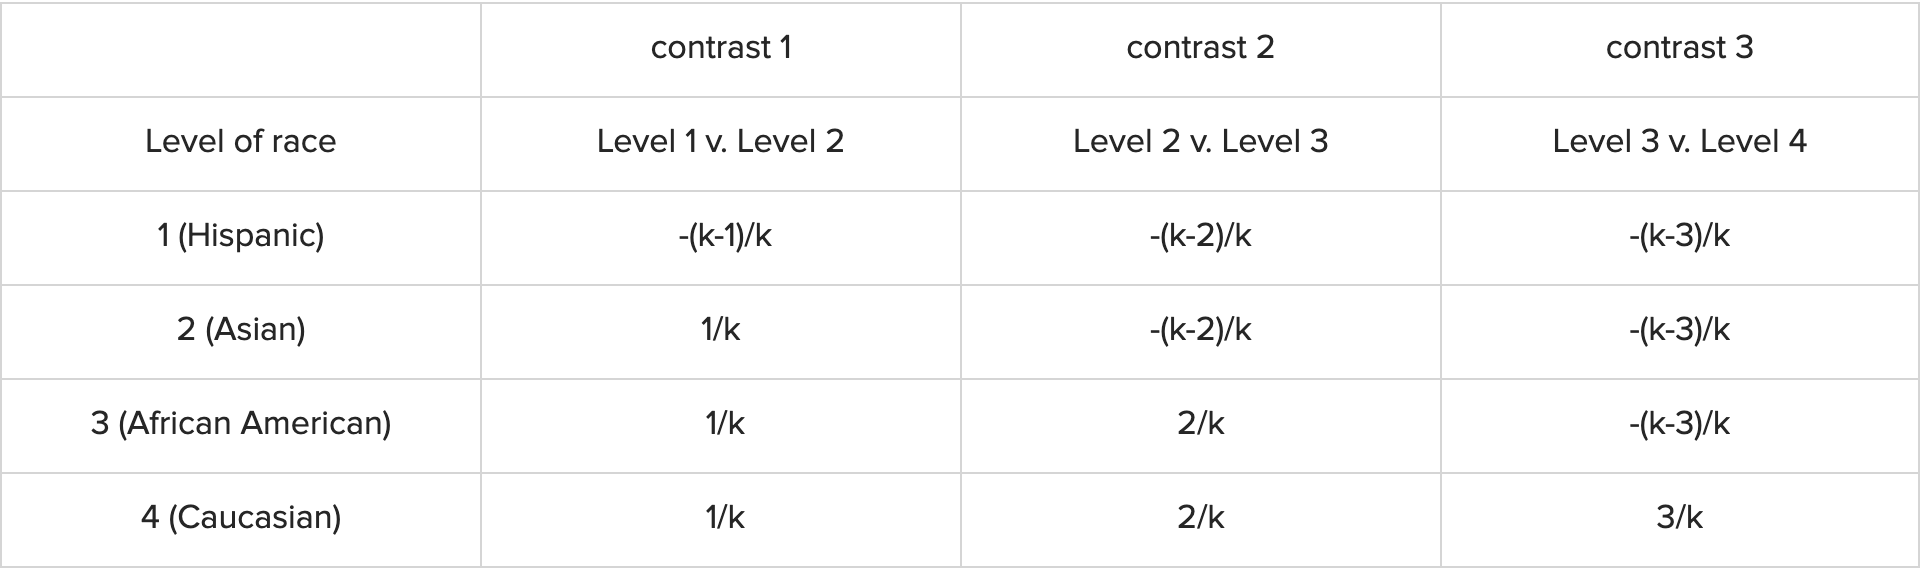
\includegraphics[scale=0.3,center]{backward.png}
    \caption{An Example of Backward Difference Encoding}
    \label{fig:backward}
\end{figure}

Another encoding method that was explored was ordinal encoding, which ensures that the encoding of the variables retains the ordinal nature of the feature. This is a very typical method of encoding, although it is best suited for ordinal categorical variables. The methodology involves assigning an integer to every distinct object in a feature column. Since our features do not have an ordinal nature, they are assigned the integer either using the order that they appear in, or using the alphabetical order of the objects \cite{ordinal}. 

The last method that we explored was base-N encoding, which encodes categorical features into arrays of a base-N representation. When N equals the number of different objects there are, this is equivalent to ordinal encoding \cite{scikit}. When $n=1$, the methodology is essentially the same as that of one-hot encoding. When $n=2$, it is essentially the same as binary encoding. One main purpose of base-N encoding is to make grid searching easier \cite{encodingcateg}.  

Grid searching is a method employed to find the optimal hyperparameters for a particular model to increase its accuracy \cite{gridsearch}. Hyperparameters are external configurations to your model whose values are not estimatable from your data. Instead, they are typically set by the practicioner, or set using heuristics and are tuned for a specific practical problem \cite{hyperparam}. Thus, when we use grid searching for a specific problem, we are tuning the hyperparameters to determine what parameters of the model will yield the most skillful predictions. 

Another method of estimating the skill of a machine learning model is cross validation, which uses a limited sample of your data to estimate how the model will perform when making predictions on non-training data. This is a commonly used method, as it typically results in a less biased prediction of the model's skill than that of a simple train/test split of your data. The methodology involves randomly splitting your data into $k$ groups, using one of the groups as a test set and the rest as a training set. It does this for all of the groups and summarizes the skill of the model based on the sample of model evaluation scores of the $k$ groups \cite{crossval}. 

\subsection{Learned Embedding}
\hspace{\parindent}Learned embedding, also known as word embedding or “embedding”, is a distributed representation of categorical data. Each category is mapped to a vector, where the properties of that specific vector will be adapted and learned by the neural network of the model \cite{3ways}. This created vector space allows individual data points with similar categorical features to be more closely related. This takes both the benefits of ordinal encoding, by allowing relationships of data points to be learned, and one-hot encoding by providing a vector representation for each category \cite{transferlearning}.  The model we utilize is based upon the model made by Jason Brownlee for Machine Learning Mastery \cite{3ways}.

Before inputting it into the model, the dataset used must be split into only categorical features for learned embedding, which is subsequently label encoded for the embedding. The model itself utilizes Keras and Tensor Flow within a Python environment to create an embedding layer $\text{M} \times \text{N}$ where M is the number of unique entries and N is an arbitrarily assigned dimension for each categorical variable. We have set N = 10 for our learned embedding model to receive baseline results. Because the dimension of each of these layers is very high, they are flattened to a $1 \times \text{(M*N)}$ vector to be concatenated together to then be processed as a Keras Dense Layer which is then processed by the neural network. This is where normalized numerical data, if present in the data set, can be re-inserted into the embedded data for the neural network to learn from. Learned embedding allows us to represent high cardinality categorical variables while utilizing low dimension embedding to preserve the relationship between the categories allowing the learned model to not rely on memorization but be able to generalize \cite{cat2vec}.

\subsection{Wide and Deep Learning}

\subsubsection{Background \& Systematic Literature Review}

\hspace{\parindent}The paper ``Wide \& Deep Learning for Recommender Systems" \cite{chengwidedeep2016} explores how wide and deep learning can be combined to maximize the results of both frameworks. In it, they introduce how the Wide \& Deep learning (WDL) framework can be used to train both feed-forward neural networks with embeddings and linear models with feature transformations, which can improve how apps are acquired on a mobile app store. 

The wide component of their model creates a generalized linear model using the features, model parameters, and bias weights. They include transformed features, including cross-product transformations, which introduces a non-linear component into the model. In the deep component, they use a feed-forward neural network, which converts high-dimensional categorical features into embedding vectors. The embedding vectors are eventually fed into the layers of a deep neural network to reduce dimensionality. When the two components are combined, the model optimizes all the parameters simultaneously by taking the wide and deep parts and the weights of their sum into account at the training time. Because this employs joint training rather than an ensemble, the wide component only needs to complement the weaknesses of the deep component, meaning that there doesn't need to be as many cross-product transformations. 
The embeddings are then concatenated together with the reduced dimension features, which yields a dense vector of high dimensionality. This is then fed into rectified linear unit (ReLU) layers and the logistic output unit. The model quality is empirically validated against that of the previous models. 

\subsubsection{Our Implementation}
\hspace{\parindent}Wide \& Deep Learning (WDL) is used as a method to bypass the need for complex feature extraction and conversion. Category encoders are implemented as a preprocessing technique where the encoded data are passed to a classification model to make a prediction. WDL functions as a fully integrated system that embeds feature encoding into the prediction model. Essentially, the structure of the manipulated feature space created by the concatenation of the wide and deep components is passed to a neural network prediction model where feature encoding is learned as the prediction model trains. The wide component is a linear model that uses a set of cross-product feature transformations to capture how interactions between different features correlate to the target variable. Similar to one-hot encoding, this greatly expands the dimensions of the feature space. The deep learning component uses a feed-forward neural network to learn dependencies within the data by expanding and repeatedly reducing the dimensions of the feature space. Generalizations are made by matching similar dependencies within the feature space. The embedded feature vectors created by the deep component are dense representations of the original data. 

In this model, WDL is implemented by Keras, an open-source neural network library written in Python. This particular model for converting categorical features to numerical ones is based on the ``Wide and Deep Learning model for Recommender Systems" built by Heng-Tze Cheng \cite{chengwidedeep2016}. Provided a dataset, the technique splits input data into numerical and categorical features. To preprocess the initial data, two transformations are applied. First, the categorical features are converted to an integer form using a label encoder. This assigns a new integer to every distinct value within a feature column. The numerical features are normalized by a simple standard scalar transformation. This normally distributes the numerical values of the dataset to prevent bias from occurring in the training model. 

Two separate methods are implemented to independently form the wide and deep components of the model. The wide component is created by applying a polynomial transformation of degree two to the previously label-encoded categorical features, thus converting the original feature space into a higher dimension. Specifically, this generates a new feature matrix containing every polynomial combination of the original feature space with degree less than or equal to two. For example, given a feature space $(a,b)$, a polynomial transformation of degree two converts this to the higher dimensional space $(1,a,b,a^2,ab,b^2)$. The process used to build the deep component for the model is more complex. Initially, the dimensions for the final categorical feature space of the deep component is set to $\frac{1}{4}$, the size of the dimensions from the original categorical feature space. The categorical features are individually embedded and flattened using imported Keras packages to formulate feature vectors for the next step. Separately, the previously normalized numerical features are scaled to a higher dimensionality through a serious of dot products. Then, the categorical feature vectors and scaled numerical feature vector are concatenated to create the input for the deep learning aspect of the model. The dimension of the combined feature space is halved in two separate actions to extract new, more informative features from the input data using the Keras deep learning framework. The size of this space is equivalent to the dimension predefined at the beginning of the deep component method. Finally, the wide and deep components of the model are concatenated to create the final feature vector used as the input to a predictive model. 

The structure of the algorithm is illustrated in the figure below where wide and deep learning is applied to the adult dataset. As shown in Figure \ref{fig:widedeep}, the eight categorical features are individually embedded and flattened while the five numerical features are stored as a single entity and scaled to a higher dimension. This creates nine total feature spaces. These feature spaces are merged into a single entity and sent through the deep learning framework. This decreases the dimensions of the dataset and completes the deep component of the algorithm. Separately, the wide component is formulated by applying a polynomial transform to the original categorical features from the adult dataset. Lastly, the wide and deep components are concatenated to achieve the final extracted feature space.
\begin{figure}[H]
    \centering
    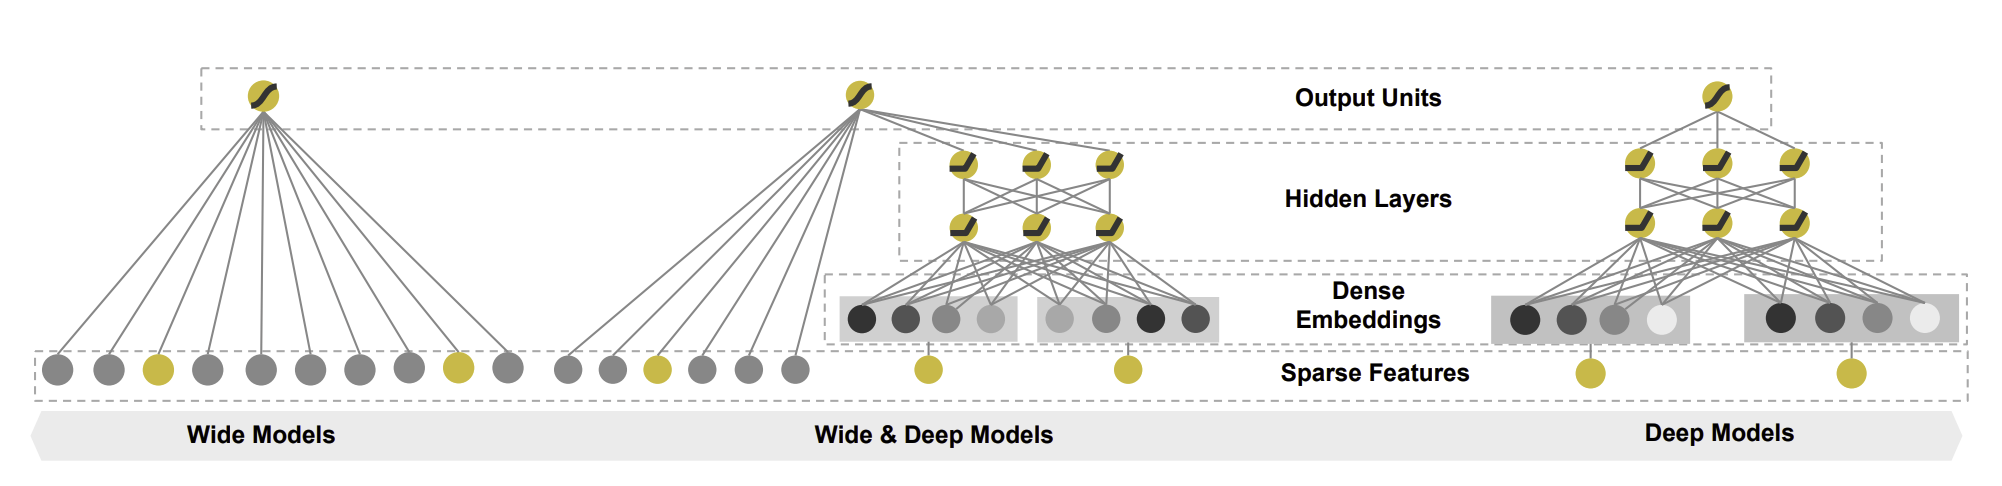
\includegraphics[scale=0.4, center]{wideanddeep.png}
    \caption{Wide and deep learning model structure}
    \label{fig:widedeep}
\end{figure}

\section{Numerical Results and Evaluation}

\hspace{\parindent}We used metrics such as accuracy, precision, recall, F-beta score, and the area under the curve (AUC) to compare the effectiveness of the algorithms. \textbf{Accuracy} quantifies the ratio of correct predictions made to the total number of predictions that an algorithm makes \cite{classificationaccuracy}. \textbf{Precision} quantifies the proportion of true positive (meaning that the algorithm correctly predicted the positive outcome) made among all positive predictions. \textbf{Recall} is the proportion of true positives made among all actual positive occurrences \cite{classificationprecisionrecall}. 

\hspace{\parindent}The \textbf{F-beta score} is a way of measuring the accuracy of a model by taking precision and recall into consideration. It is defined as 
    \begin{equation*}
        F_\beta = (1+\beta^2)\cdot\frac{\mathrm{precision\cdot    \mathrm{recall}}}{(\beta^2\cdot\mathrm{precision}+\mathrm{recall})}.
    \end{equation*} 
To give more weight to precision, we use a beta value between 0 and 1. To give more weight to recall, we use a beta value from 1 to positive infinity. When beta = 1, we have the harmonic mean, which is the point where precision and recall are weighted about the same \cite{fbeta}. Although we were not able to implement this, it is a particularly useful metric in ascertaining which model predicts classes best.

\hspace{\parindent}The \textbf{AUC}, or area under the curve, measures the area under the curve generated by plotting the true positive rate against the false positive rate on different classification thresholds. This provides an aggregate measure of the performance of the algorithm across all the possible classification thresholds. This is useful because the AUC is scale-invariant, meaning that it measures how well the predictions are ranked, and it is classification-threshold-invariant, meaning that it measures the quality of the model's predictions regardless of which classification threshold is used \cite{classificationaucroc}. 

\begin{table}[H]
\caption{OHE Random Forest Results} \label{tab:OHErf}
\begin{center}
\begin{tabular}{|c|c|c|c|c|c|}
\hline
Dataset & Subset & Accuracy & Precision & Recall & F-Beta \\ \hline
Amazon & Test & 94.08\% & 0.9408 & 1 & 0.9695 \\ \hline
 & Train & 94.26\% & 0.9462 & 1 & 0.9704 \\ \hline
US Census & Test & 99.99\% & 0.999 & 1 & 0.999 \\ \hline
 & Train & 99.99\% & 0.999 & 1 & 0.999 \\ \hline
\end{tabular}
\end{center}
\end{table}

\begin{table}[H]
\caption{OHE Decision Tree Results} \label{tab:OHEdt}
\begin{center}
\begin{tabular}{|c|c|c|c|c|c|}
\hline
Dataset & Subset & Accuracy & Precision & Recall & F-Beta \\ \hline
Amazon & Test & 94.08\% & 0.9408 & 1 & 0.9695 \\ \hline
 & Train & 94.56\% & 0.9479 & 0.9971 & 0.9718 \\ \hline
US Census & Test & 100\% & 1 & 1 & 1 \\ \hline
 & Train & 100\% & 1 & 1 & 1 \\ \hline
\end{tabular}
\end{center}
\end{table}

\begin{table}[H]
\caption{Comparison of Different Encoding Methods for Adult Dataset}
\label{tab:adCOM}
\begin{center}
\begin{tabular}{|c|c|c|c|c|c|c|c|c|}
\hline
 & One-Hot & Ordinal & \begin{tabular}[c]{@{}l@{}}Backward\\ Difference\end{tabular} & Base 1 & Base 2 & Base 5 & Base 10 & Binary \\ \hline
Accuracy & \textbf{0.8571} & 0.8567 & 0.8567 & \textbf{0.8571} & 0.8533 & 0.8566 & \textbf{0.8587} & 0.8533 \\ \hline
Precision & 0.7301 & 0.7407 & 0.7407 & 0.7302 & 0.7356 & 0.7489 & 0.7585 & 0.7356 \\ \hline
Recall & 0.6266 & 0.6053 & 0.6053 & 0.6269 & 0.5918 & 0.5897 & 0.5897 & 0.5918 \\ \hline
\end{tabular}
\end{center}
\end{table}

\begin{table}[H]
\caption{Learned Embedding Results} \label{tab:LearnedEmbed}
\begin{center}
\begin{tabular}{|c|c|c|c|c|}
\hline
Dataset & Accuracy & Precision & Recall & F-Beta \\ \hline
Adult & 83.31\% & - & - & - \\ \hline
US Census & 99.99\% & - & - & - \\ \hline
KDD & 98.44\% & - & - & - \\ \hline
Amazon & 98.55\% & - & - & - \\ \hline
\end{tabular}
\end{center}
\end{table}

\begin{table}[H]
\caption{Adult Dataset (Wide and Deep)} \label{tab:adWD}
\begin{center}
\begin{tabular}{|c|c|c|c|c|} \hline
 & Accuracy & Precision & Recall & F-Beta \\ \hline
train & 82.64\% & - & - & -\\ \hline
\end{tabular}
\end{center}
\end{table}

In tables \ref{tab:OHErf} and \ref{tab:OHEdt}, we observe significantly high values for all our metrics. This is most likely due to the high-frequency data entries. When there are high cardinality categorical variables, using one-hot encoding is not ideal because the encoding method typically has trouble with memorization \cite{encodingcateg}. Additionally, the high performance of the US Census dataset in both one-hot encoding and learned embedding may point to some characteristic of the specific dataset that is causing to perform so well for both these methods.

In table \ref{tab:adCOM}, we compared the metrics obtained when encoding the Adult dataset using different methods and running it using random forest on optimized hyperparameters. We decided to focus on the accuracy metric as a preliminary way to evaluate the effectiveness of our encoding methods. Here, one-hot encoding and base-10 encoding appear to be more effective at predicting outcomes than the other methods employed. Base-1 is highlighted as well, but in base-N encoding, this should be similar to one-hot encoding \cite{encodingcateg}. The results for base-10 encoding are most likely so high because the N chosen is so close to the number of categorical features in the Adult dataset. Thus, it appears that one-hot encoding is the best method of all of these, which makes sense, as all the other methods ordinally encode the features. Thus, when the algorithm evaluates the data and makes a prediction, it is still treating the variables as though they are ordinal variables, while one-hot encoding prevents this. 

WDL reaps the advantages of both linear and deep learning models by combining them into a single hybrid system. Linear models are good at ``memorizing" specific feature combinations but poor at making generalizations across feature columns. Deep learning models can sometimes be prone to over-generalization when creating the new feature space based on discovered dependencies within the data. By combining both types of models, WDL tends to perform well on larger datasets with high-cardinality features. Note that one-hot encoding is the opposite. Therefore, WDL can shine where traditional category encoders tend to fail. Tested on Adult, WDL model obtained an accuracy of 82.58\%, whereas one-hot encoding achieved an accuracy of 85.71\%. Adult is the smallest dataset where only one column can be considered to have relatively high cardinality with a frequency of around 20,000. It is noted that, in terms of WDL, high-cardinality means each feature has closer to millions/billions of unique values \cite{github}. Therefore, it makes sense that one-hot encoding performed better than WDL when tested on the adult dataset. As a final remark, it is somewhat difficult to compare the results of WDL and learned embedding to other encoding methods because they are not tested on the same classification model. Other deep learning models that can independently be used for feature extraction and conversion will be investigated in order to easily compare results by using the same classification models for predictions.

\section{Conclusion}

\hspace{\parindent}By the above results, we may conclude one-hot encoding proves to be more effective on datasets that do not contain high-cardinality features, whereas deep learning based networks perform better on datasets with high-cardinality features. It was difficult to compare the actual metrics of these methods however, due to the fact that WDL and learned embedding directly gives us results, while our other encoding methods had to be encoded separately and then run on a machine learning algorithm. One recommendation would be to parse through a dataset to evaluate the cardinality of the features to then determine which encoding method or learning algorithm would be best. Methods that can lead to improvements to machine learning results are valuable for creating efficient algorithms and allow for further progress in data science. This research may lead toward more accurate machine learning algorithms and implementations, but it may also act as a guideline to which encoding method is best for a particular situation.

\bibliographystyle{plain}
\bibliography{bibliography}

\end{document}